The experiment is a fixed suite of 64 labelled inputs, with three repetitions per input and method (384 calls). We kept every generated input. The 28 named inputs comprise 14 examples chosen to exercise the stated branches and 14 parameters $t=-5,0,1,2,3,4,10,11,32,33,128,129,1000,1001$ of the alternating line. Using Python's pseudorandom generator with seed $20261009$, we also draw 24 independent six-tuples uniformly from $[-3,3]^6$. Finally, 12 planted MA inputs are obtained by drawing all six nonnegative topological entries uniformly from $\{0,1,2\}$ and applying six independent uniformly chosen mutations. The exact draws and generating words are saved.

Runs used an Apple M1 CPU (8 cores, 16 GiB RAM), macOS 26.3 on arm64, and CPython 3.9.6. The program is single-process. For each input the method order is hybrid/search, search/hybrid, hybrid/search. One acyclic warm-up call precedes measurement; there is no result cache. The finite-orbit table is built and checked at import. Each named call is capped at 100,000 discovered states or 3 seconds; each generated call at 25,000 states or 1 second. Timeouts are cooperative, checked once per BFS expansion (and during iterative witness construction). A state cap can therefore be reached before a time cap. Such runs return UNKNOWN.

Timing uses \code{perf_counter} inside the diagnostic call, including the calculation of $H$, tests, search and independent positive-witness replay. It excludes imports and file I/O. Discovered states and expanded states count only BFS states; shortcut-only calls report zero. Mutation evaluations count candidates in BFS, rank-three descent and iterative line reduction, including duplicate or out-of-box candidates. Fixed-word criteria construct their words directly. Witness replay mutations are a separate counter. These conventions explain, for example, why a positive fixed-word shortcut can have zero counted candidate mutations.

\begin{table}[htbp]\centering\scriptsize
\caption{Selected named inputs. Times are medians of three runs, in milliseconds. The full minimum/median/maximum values, expanded states and witness-replay counts are in the saved summary. $S$ and $E$ are discovered states and candidate mutations for search alone. A star means UNKNOWN at the state cap; the displayed time is time spent, not completion time. All hybrid calls in this table complete.}\label{tab:named}
\begin{tabular}{@{}lcrrrrrr@{}}\toprule
Input & Hybrid branch & $H$ & $\log_{10}N$ & Hybrid ms & Search ms & $S$ & $E$\\\midrule
Acyclic & acyc. & 59 & 12.5 & 0.026 & $0.025$ & 0 & 0 \\
Disconnected + & disc. & 109 & 14.0 & 0.113 & $0.114$ & 7 & 9 \\
Disconnected -- & tri. & 78 & 13.2 & 0.025 & $0.064$ & 2 & 8 \\
Double box & box & 72 & 13.0 & 0.182 & $14.341$ & 726 & 2,904 \\
Finite orbit & orbit & 59 & 12.5 & 0.028 & $0.464$ & 24 & 96 \\
$s_1$ & proper & 71 & 12.9 & 0.090 & $440.812$ & 22,896 & 91,584 \\
$s_3$ & proper & 71 & 12.9 & 0.101 & $439.053$ & 22,896 & 91,584 \\
Five + & five & 362 & 17.2 & 0.044 & $0.048$ & 2 & 1 \\
Five -- & five & 295 & 16.6 & 0.038 & $1996.809$ & 89,856 & 359,424 \\
Product & prod. & 439 & 17.7 & 0.056 & $0.147$ & 11 & 12 \\
Quadratic & quad. & 442 & 17.7 & 0.046 & $0.072$ & 5 & 4 \\
Scalar equality & proper & 97 & 13.7 & 0.186 & $270.536$ & 13,020 & 52,080 \\
Search positive & BFS & 80 & 13.2 & 0.191 & $0.058$ & 4 & 3 \\
$q(10)$ & line & 20,066 & 27.6 & 0.081 & $1.397$ & 102 & 234 \\
$q(11)$ & line & 29,352 & 28.6 & 0.031 & $1513.910^{*}$ & 100,000 & 284,309 \\
$q(128)$ & line & 536,871,450 & 54.2 & 0.548 & $77.486$ & 4,093 & 15,449 \\
$q(129)$ & line & 553,846,304 & 54.3 & 0.038 & $1228.819^{*}$ & 100,000 & 205,593 \\
$q(1000)$ & line & 2,000,000,004,026 & 75.6 & 3.840 & $712.278$ & 33,619 & 131,933 \\
$q(1001)$ & line & 2,008,012,012,032 & 75.6 & 0.043 & $1557.634^{*}$ & 100,000 & 281,707 \\
\bottomrule\end{tabular}\end{table}
The branch abbreviations denote acyclicity, disconnected descent, a rank-three obstruction, the double-box certificate, the finite closed orbit, proper-order exclusion, the line formula, the five-parameter criterion, the product and quadratic criteria, and bounded BFS, respectively. Every reported MA witness was also replayed after the experiment with a separate dense-matrix implementation. Completed labels agree between methods.

\begin{table}[htbp]\centering\small
\caption{All inputs, aggregated by sample. Time is the median of the three sums over the sample, in seconds. State and mutation columns sum the per-input medians. UNKNOWN calls are retained.}\label{tab:generated}
\begin{tabular}{llrrrrrr}\toprule
Sample & Method & MA & NMA & Unknown & Time (s) & States & Mutations\\\midrule
Named & hybrid & 15 & 13 & 0 & 0.0063 & 4 & 600 \\
Named & search & 15 & 9 & 4 & 12.9275 & 710,931 & 2,234,099 \\
Uniform & hybrid & 16 & 8 & 0 & 0.6070 & 30,146 & 120,538 \\
Uniform & search & 16 & 7 & 1 & 1.5973 & 77,946 & 309,310 \\
Planted & hybrid & 12 & 0 & 0 & 0.0051 & 299 & 606 \\
Planted & search & 12 & 0 & 0 & 0.0042 & 299 & 606 \\
\bottomrule\end{tabular}\end{table}

The hybrid method resolves all 64 inputs under these limits. Search alone resolves 59; four named inputs and one uniform draw reach their state caps in all repetitions. All 12 planted inputs are confirmed MA by both methods. This sample is small and deliberately includes structured cases; it is not an estimate of the proportion of MA quivers or of average complexity under a canonical distribution.

The contrast is especially clear for the two negative seeds: each has 22,896 states in its reachable height-bounded component, whereas the hybrid proof only inspects its six cyclic orders. For $q(1000)$ the line witness has 500 mutations and must be constructed and checked; its running time consequently grows with the witness length. The odd-line negative certificate does not construct such a trajectory. This is a difference in output work as well as search avoidance. The a priori state bound remains vastly larger than the explored components, including on inputs where BFS is required. It proves termination but is a poor practical predictor of runtime.

\begin{figure}[htbp]\centering
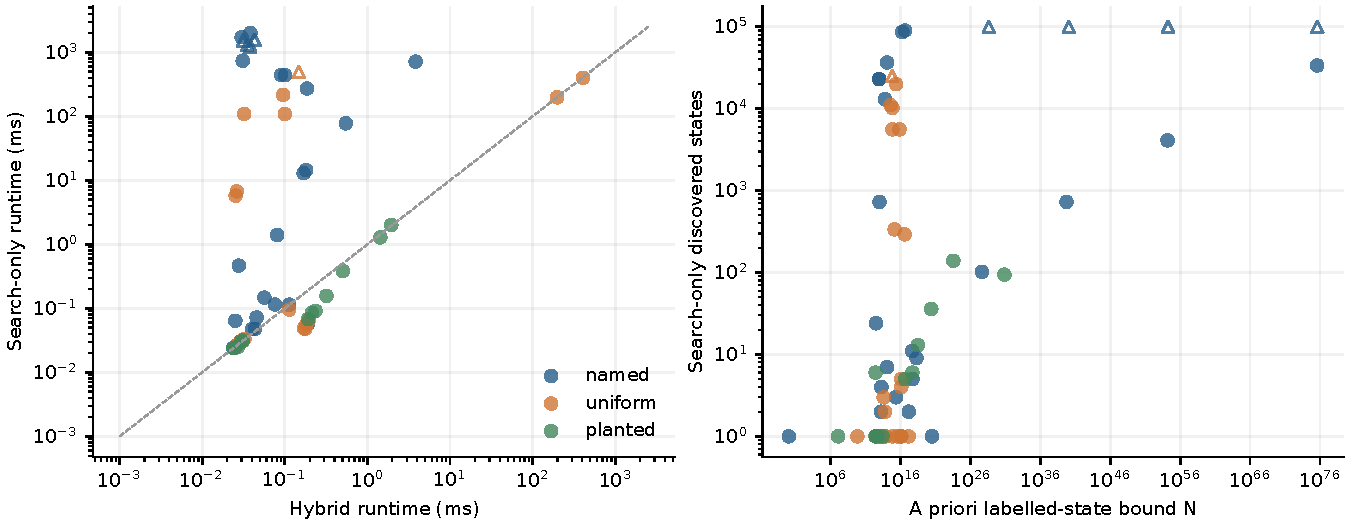
\includegraphics[width=\textwidth]{figures/performance.pdf}
\caption{Each marker represents one of the 64 inputs (medians of three calls). Left: paired runtimes; open upward triangles denote capped search-only runs and must not be read as completion times. The diagonal marks equal time. Right: discovered search-only states versus the labelled bound $N$; capped runs are open triangles. An initially acyclic input has zero BFS states, displayed here at one solely for the logarithmic axis.}\label{fig:performance}
\end{figure}
The plotting environment uses Python 3.12.14 and Matplotlib 3.10.7; its dependency lock is separate from the standard-library-only classifier. Tables and the figure are generated from the saved raw measurements, not from timings in the review report.
